% !TeX spellcheck = en_US
% !TEX root = ../thesis-example.tex
%
\section{Additional Camera Stencil}

When producing on small and / or amateur sets, there are usually constraints to 
size and proportions of the green screen production, thus limiting the 
record-able space. Since a calibrated play space can be fetched from the 
SteamVR API to receive a proper-sized bounding box, it is possible to do a 
projection of the green screens real size inside a virtual scene and use this 
as a stencil for the incoming video feed, effectively cropping off around all 
edges outside of a calibrated green screen. This means that a real world camera 
can film outside the edges of a green screen, recorded pixels beyond the green 
box are getting discarded and it will not degrade the visual performance of the 
image composition.

\begin{figure}[htb]
	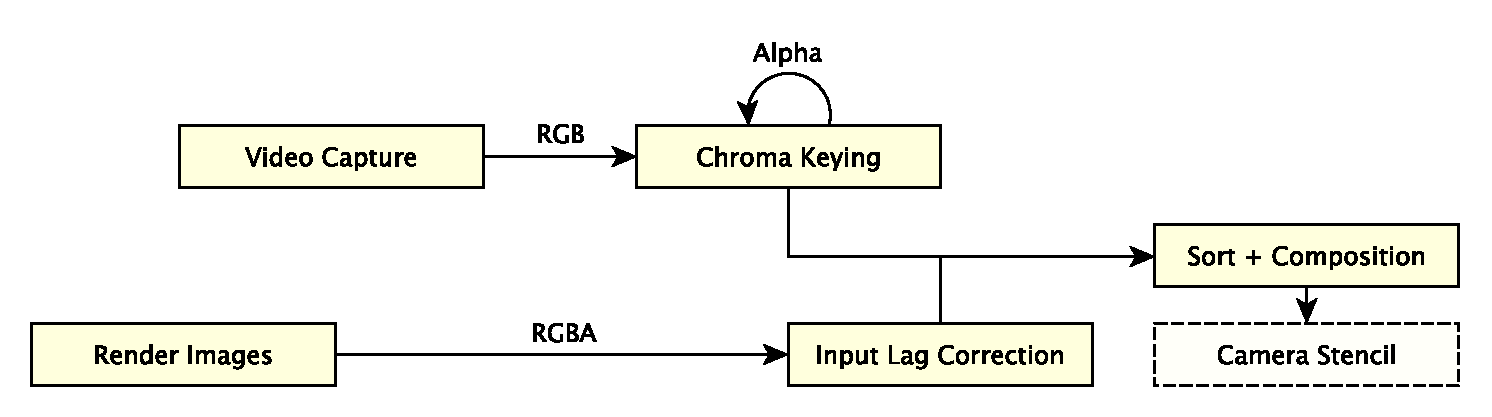
\includegraphics[width=\textwidth]{_raw_resources/pipeline_steps/4_6_stencil.pdf}
	\caption{After sorting the scene additional stenciling of the video feed is 
	necessary}
	\label{fig:steps:stencil}
\end{figure}

A virtual projection can be seen in figure \ref{fig:stencil:projection} with 
reconstructed camera parameters. With help of Unitys' engine-editor a 
green screen can be calibrated and should match very closely to all real world 
parameters, allowing a real world camera to film over the edges of a 
green screen without destroying the image composition. If a VR actor is outside 
of the chroma key planes, the resulting image composition wouldn't be usable, 
thus this solution enhances a composed image without major 
drawbacks.

\todo{Might need additional text for clarifying}

\begin{figure}[htbp]
	\caption[Some Argument]{Virtual projection and photo of VR actor - red 
	colored areas will be cut off}
	\label{fig:stencil:projection}
	\begin{subfigure}[t]{.3\textwidth}
		\centering
		\includegraphics[width=\textwidth]{gfx/stencil/virtual.png}
		\caption{Virtual reprojection of a calibrated green screen}
	\end{subfigure}
	\begin{subfigure}[t]{.3\textwidth}
		\centering
		\includegraphics[width=\textwidth]{gfx/stencil/img.png}
		\caption{Masking what would be remaining video content}
	\end{subfigure}
	\begin{subfigure}[t]{.3\textwidth}
		\centering
		\includegraphics[width=\textwidth]{gfx/stencil/scene.png}
		\caption{Composition after stencil has been applied}
	\end{subfigure}
	\label{fig:virtual-proj-stencil}
\end{figure}

In-engine this setup is a simple addition: After registering another virtual 
camera to the camera manager it is used to simply render green planes where the 
real world green screen is placed. Taken from previous projection parameters in 
\ref{sec:projection-params} this virtual camera receives a dedicated culling 
mask which only contains all green box projection planes. All other cameras 
ignore this layer and are therefore invisible for any composing camera. After 
each drawn frame, Unity is able to clear the frame buffer with an alpha color 
as 0 - all remaining fragments from the green box write any color with an alpha 
as 1; the color compartment is discarded and will not be used further. This 
creates a lookup texture where an alpha-mask is rendered which will be 
transferred to the video feeds alpha (see figure 
\ref{fig:virtual-proj-stencil}).

We have now achieved a green box projection inside the same scene without any 
complex management processes needed in Unity. Due to the quick setup it works 
well for fast calibration and allows for a broad camera angle up to the green 
screens edges without degrading the mixed reality performance. Recording beyond 
these edges will yield into a composition of front and background renderings 
since all camera pixels will be completely discarded.
\newline
Unfortunately stencil-operations are poorly documented in Unity and add an 
overhead which cannot be measured from built in profiler tools - as such it 
adds unknown performance costs and have not been used in this thesis, hence the 
fall back of rendering an alpha map.